\documentclass[11pt,letterpaper]{article}
\usepackage{naaclhlt2010}
\usepackage{times}
\usepackage{latexsym}
\usepackage{amsmath,amsthm, amssymb}
\usepackage{multirow}
\usepackage{microtype}
\usepackage{subfigure}
\usepackage{bm}
\usepackage{graphicx}
\usepackage{graphics}
\usepackage{bm}
\usepackage{multirow}
\usepackage{dsfont}

%%%% EVIL %%%%%%
\usepackage[compact,small]{titlesec}
\usepackage[small]{caption}
\usepackage{mdwlist}

\renewcommand{\topfraction}{0.95}
\renewcommand{\textfraction}{0.05}
\renewcommand{\floatpagefraction}{0.95}

\setlength{\abovecaptionskip}{0pt}

%\setlength{\belowcaptionskip}{0pt}
\setlength{\textfloatsep}{8pt}
%\setlength{\floatsep}{0pt}
%%%% EVIL %%%%%%

\newcommand{\myfig}[1]{Figure~\ref{#1}}
\newcommand{\myeq}[1]{Equation~\ref{#1}}
\newcommand{\mytab}[1]{Table~\ref{#1}}
\newcommand{\wordset}[1]{\texttt{\{#1\}}}
\newcommand{\word}[1]{\texttt{#1}}
\newcommand{\mysec}[1]{Section~\ref{#1}}

%%% Temporary
%\usepackage{fancyhdr}
%\chead{{\bf DRAFT COPY: DO NOT CITE OR DISTRIBUTE}}
%\lhead{}
%\rhead{}
%\pagestyle{fancy}

\title{Not-So-Latent Dirichlet Allocation: \\ 
       Collapsed Gibbs Sampling Using Human Judgments}

\author{}

\begin{document}

%% \makeanontitle
\maketitle
\vspace{-.1in}
\begin{abstract}%
  Probabilistic topic models are a popular tool for the unsupervised
  analysis of text, providing both a predictive model of future text
  and a latent topic representation of the corpus.  Recent studies
  have found that while there are suggestive connections between topic
  models and the way humans interpret data, these two often disagree.
  In this paper, we explore this disagreement from the perspective of
  the learning process rather than the output.  We present a novel
  task, \emph{tag-and-cluster}, which asks subjects to simultaneously
  annotate documents and cluster those annotations.  We use these
  annotations as a novel approach for constructing a topic model,
  grounded in human interpretations of documents.  We demonstrate that
  these topic models have features which distinguish them from
  traditional topic models.
\end{abstract}

\section{Introduction}
Probabilistic topic models have become popular tools for the
unsupervised analysis of large document
collections~\cite{deerwester-90,griffiths02probabilistic,blei-09}.
These models posit a set of latent \emph{topics}, multinomial
distributions over words, and assume that each document can be
described as a mixture of these topics.  With algorithms for fast
approxiate posterior inference, we can use topic models to discover
both the topics and an assignment of topics to documents from a
collection of documents.  (See \myfig{fig:nyttopics:big}.)

These modeling assumptions are useful in the sense that, empirically,
they lead to good models of documents.  They also anecdotally
lead to semantically meaningful decompositions of them: topics tend to
place high probability on words that represent concepts, and documents
are represented as expressions of those concepts.  Perusing the
inferred topics is effective for model verification and for ensuring
that the model is capturing the practitioner's intuitions about the
documents.  Moreover, producing a human-interpretable decomposition of
the texts can be a goal in itself, as when browsing or summarizing a
large collection of
documents.
\cite{Chang:2009fk}

In this spirit, much of the literature comparing different topic
models presents examples of topics and examples of document-topic
assignments to help understand a model's mechanics.  Topics also can
help users discover new content via corpus
exploration~\cite{mimno-07a}.  The presentation of these topics
serves, either explicitly or implicitly, as a qualitative evaluation
of the latent space, but there is no explicit \emph{quantitative}
evaluation of them.  Instead, researchers employ a variety of metrics
of model fit, such as perplexity or held-out likelihood.  Such
measures are useful for evaluating the predictive model, but do not
address the more explatory goals of topic modeling.

In this paper, we present a method for measuring the
interpretatability of a topic model.  We devise two human evaluation
tasks to explicitly evaluate both the quality of the topics inferred
by the model and how well the model assigns topics to documents.  The
first, \emph{word intrusion}, measures how semantically ``cohesive''
the topics inferred by a model are and tests whether topics correspond
to natural groupings for humans.  The second, \emph{topic intrusion},
measures how well a topic model's decomposition of a document as a
mixture of topics agrees with human associations of topics with a
document.  We report the results of a large-scale human study of these
tasks, varying both modeling assumptions and number of topics.  We
show that these tasks capture aspects of topic models not measured by
existing metrics and--surprisingly--models which achieve better
predictive perplexity often have less interpretable latent spaces.

\section{Topic models and Inference}
\label{sec:models}

% Topic models discover patterns of word usage in a corpus.  Related
% words often appear in similar documents, and topic models can discover
% clusters of words that share context.  Because words in these clusters
% often seem to ``make sense'' together, they are described as topics.
% For illustration, three topics from a topic model called latent
% Dirichlet allocation (LDA)~\cite{blei-03} are shown in
% Figure~\ref{fig:nyttopics:topic}.

% Topic models are unsupervised; they do not require labels or
% annotations.  Instead, they discover latent topics directly from the
% data.  In addition to finding topics, topic models also assign
% mixtures of these topics to documents.  This is illustrated in
% Figure~\ref{fig:nyttopics:doc}. 

% We restrict ourselves to exchangeable topic models, in which the order
% of the words within a document does not matter.  The models we
% consider are also probabilistic, in the sense that they seek to
% approximate the vector of observed word counts as a mixture of topic
% distributions; fitting one of these topic models entails finding a
% point on the topic simplex that best describes the document.

Topic models posit that each document is expressed as a mixture of
topics.  These topic proportions are drawn once per document, and the
topics are shared across the corpus.  In this paper we consider Latent
Dirichlet allocation (LDA)~\cite{blei-03} a topic model which treats
each document's topic assignment as a multinomial random variable
drawn from a symmetric Dirichlet and logistic normal prior,
respectively.

Inference algorithms for all of these topic models build the same type
of latent space: a collection of topics for the corpus and a
collection of topic proportions for each of its documents.  While this
common latent space has explored for over two decades, its
interpretability remains unmeasured.

\begin{figure*}[t]
\centering
\subfigure[Topics]{
  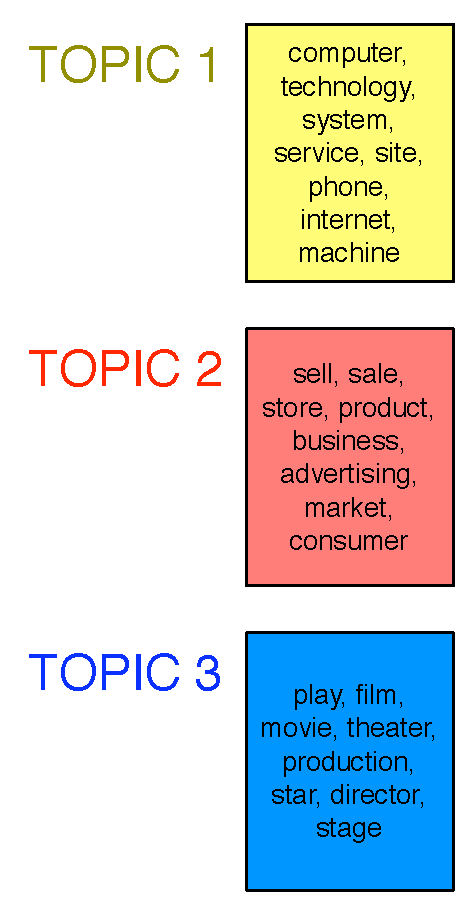
\includegraphics[scale=0.35]{figures/nyt_topics.pdf}
  \label{fig:nyttopics:topic}
}
\hspace{0.4in}
\subfigure[Document Assignments to Topics]{
  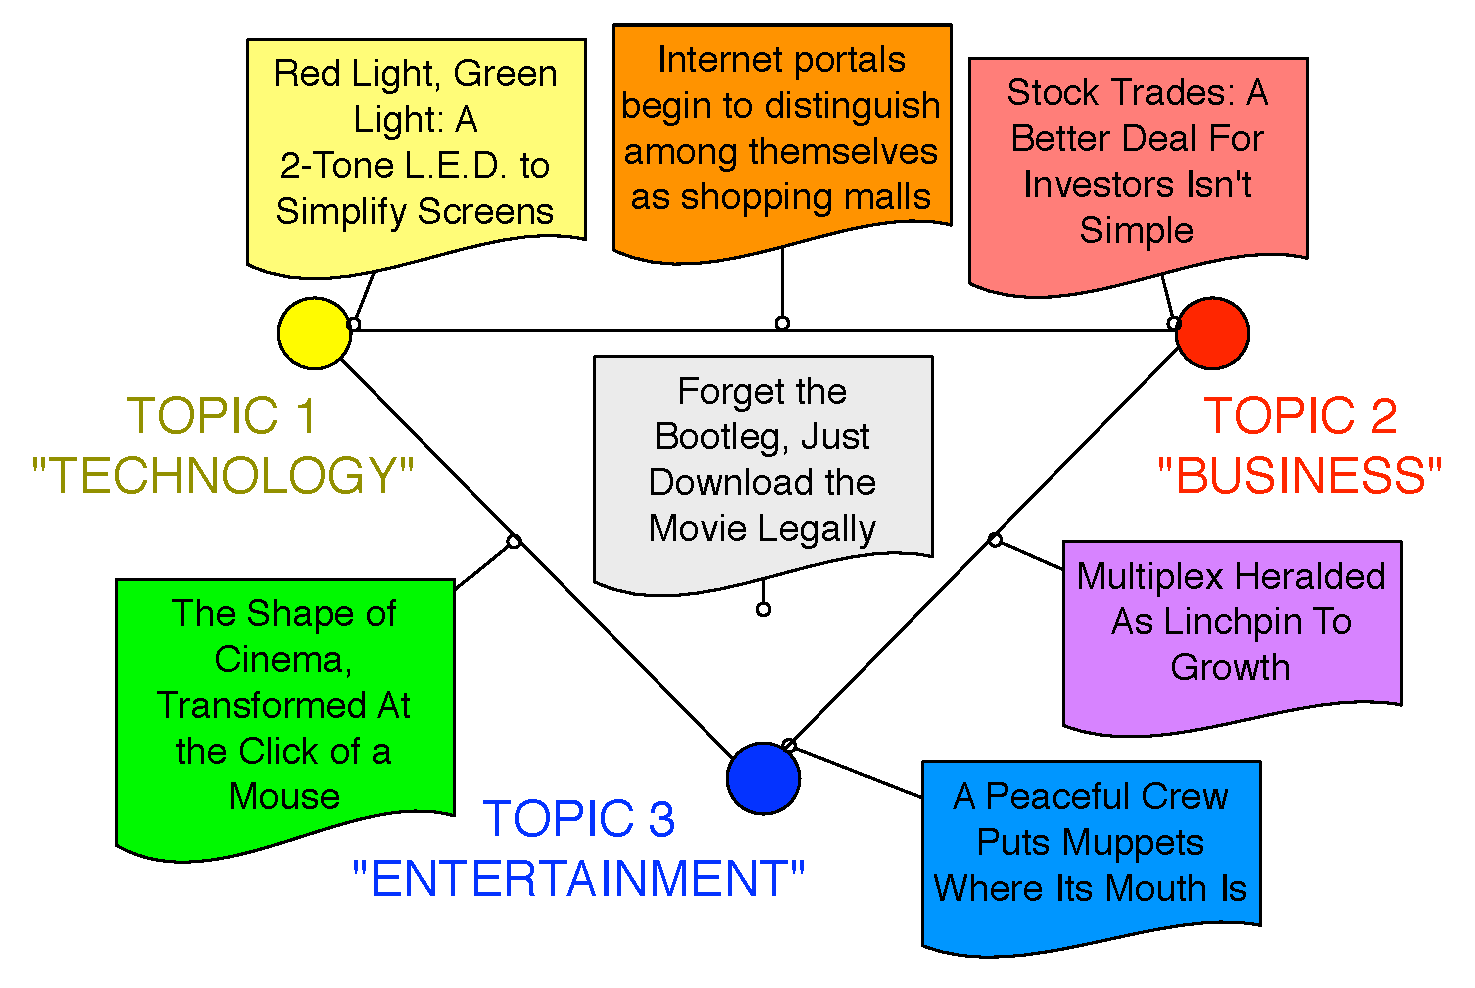
\includegraphics[scale=0.35]{figures/nyt_documents.pdf}
  \label{fig:nyttopics:doc}
}
\caption{The latent space of a topic model consists of topics,
  which are distributions over words, and a distribution over these
  topics for each document.  On the left are three topics from a
  fifty topic LDA model trained on articles from the New York
  Times.  On the right is a simplex depicting the distribution
  over topics associated with seven documents.  The line from each
  document's title shows the document's position in the topic
  space.}
\label{fig:nyttopics:big}
\end{figure*}

\begin{figure}[t]
\centering
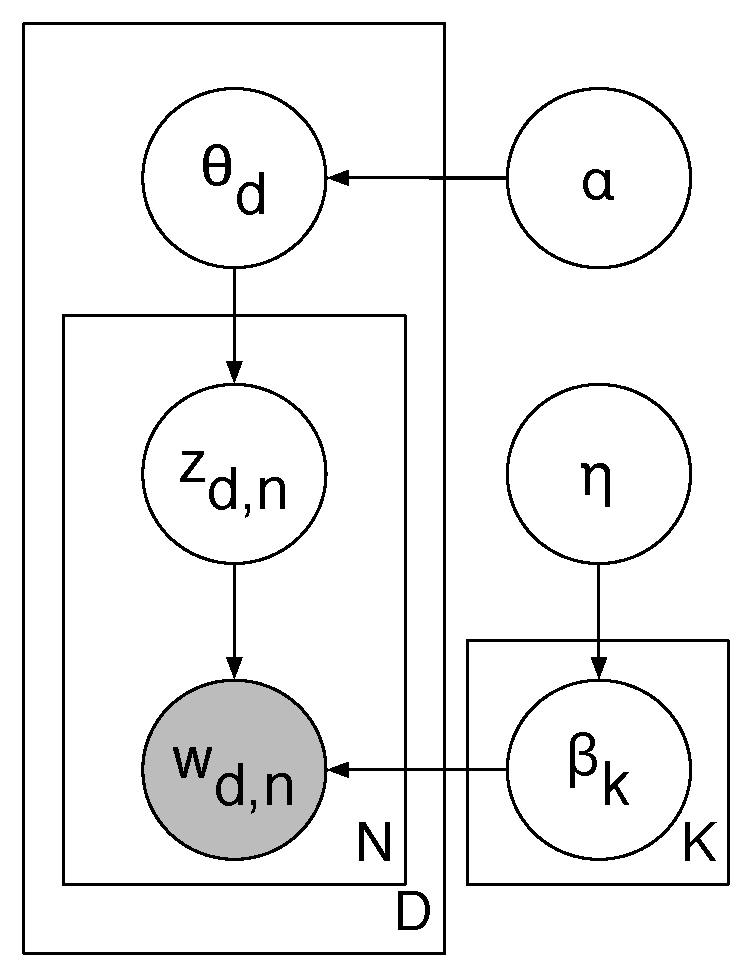
\includegraphics[width=0.5\linewidth]{figures/lda}
\caption{A graphical model depiction of latent Dirichlet allocation
  (LDA).  Plates denote replication.  Shaded circles denote observed
  variables and unshaded circles denote hidden variables.}
\label{fig:lda}
\end{figure}

Formally, the generative process of LDA is as follows:
\begin{enumerate*}
  \item For each topic $k$, 
    \begin{enumerate*}
    \item Draw topic $\beta_k \sim \mathrm{Dir}(\eta)$
    \end{enumerate*}
  \item For each document $d$, 
    \begin{enumerate*}
    \item Draw topic proportions $\theta_d \sim \mathrm{Dir}(\alpha)$
    \item For each word $w_{d, n}$, 
      \begin{enumerate*}
      \item Draw topic assignment $z_{d,n} \sim \mathrm{Mult}(\theta_d)$
      \item Draw word $w_{d,n} \sim \mathrm{Mult}(\beta_{z_{d,n}})$
      \end{enumerate*}
    \end{enumerate*}
\end{enumerate*}
The parameters of the model are the number of topics, $K$, as well as
the Dirichlet priors on the topic-word distributions and
document-topic distributions, $\alpha$ and $\eta$.  The only observed
variables of the model are the words, $w_{d,n}$.  The remaining
variables must be inferred.

There are several techniques for performing posterior inference,
i.e., inferring the distribution over hidden variables given a
collection of documents, including variational
inference~\cite{blei-03} and Gibbs sampling~\cite{griffiths-06}.  In
the sequel, we focus on the latter approach.  

Collapsed Gibbs sampling for LDA treats the topic-word and
document-topic distributions, $\theta_d$ and $\beta_k$, as nuisance
variables to be marginalized out. The posterior distribution over the
remaining latent variables, the topic assignments $z_{d,n}$, can be
expressed as
\begin{eqnarray*}
  &&p(\bm{z} | \alpha, \eta, \bm{w}) \propto \\
  &&\qquad \prod_{d}\prod_{k} \left[ \Gamma(n_{d,k} + \alpha_{k})\frac{\Gamma(\eta_{w_{d,n}} + n_{w_{d,n}, k})}{\Gamma(\sum_w n_{w, k} + \eta_w)}\right],
\end{eqnarray*}
where $n_{d,k}$ denotes the number of words in document $d$ assigned
to topic $k$ and $n_{w,k}$ the number of times word $w$ is assigned to
topic $k$.  This leads to the sampling equations,
\begin{eqnarray}
  &&p(z_{d,i} = k | \alpha, \eta, \bm{w}, \bm{z}y) \propto \\
  &&\qquad (n^{\lnot d,i}_{d,k} + \alpha_{k})\frac{\eta_{w_{d,i}} + n^{\lnot d,i}_{w_{d,i}, k}}{\sum_w n^{\lnot d,i}_{w, k} + \eta_w},
  \label{eq:sampling}
\end{eqnarray}
where the superscript $\lnot d,i$ indicates that these statistics
should exclude the current variable under consideration, $z_{d,i}$.

In essence, the model performs inference by looking at each word in
succession, and probabilistically assigning it to a topic according to
\myeq{eq:sampling}.  \myeq{eq:sampling} is derived through the
modeling assumptions and choice of parameters.  Now the question is,
when humans are given a similar assignment, to assign words to
clusters, will their own sampling equations follow \myeq{eq:sampling}
or will they be different, reflecting different underlying assumptions
about the data.

For models that use held-out likelihood, Wallach et
al.~\cite{wallach-09} provide a summary of evaluation
techniques. These metrics borrow tools from the language modeling
community to measure how well the information learned from a corpus
applies to unseen documents.  These metrics generalize easily and
allow for likelihood-based comparisons of different models or
selection of model parameters such as the number of topics.  However,
this adaptability comes at a cost: these methods only measure the
probability of observations; the internal representation of the models
is ignored.

Griffiths et al.~\cite{griffiths-06} is an important exception to the
trend of using external tasks or held-out likelihood.  They showed
that the number of topics a word appears in correlates with how many
distinct senses it has and reproduced many of the metrics used in the
psychological community based on human performance.  However, this is
still not a deep analysis of the structure of the latent space, as it
does not examine the structure of the topics themselves.

We emphasize that not measuring the internal representation of topic
models is at odds with their presentation and development.  Most topic
modeling papers display qualitative assessments of the inferred topics
or simply assert that topics are semantically meaningful, and
practitioners use topics for model checking during the development
process.  This implicit notion that topics have semantic meaning for
users has even motivated work that attempts to automatically label
topics~\cite{mei-07}.  Our goal is to measure the success of
interpreting topic models across number of topics and modeling
assumptions.

\section{Using human judgments to examine the topics}
\label{sec:tasks}
Although there appears to be a longstanding assumption that the latent
space discovered by topic models is meaningful and useful, evaluating
such assumptions is difficult because discovering topics is an
unsupervised process.  There is no gold-standard list of topics to
compare against for every corpus.  Thus, evaluating the latent space
of topic models requires us to gather exogenous data.

In this section we propose two tasks that create a formal setting
where humans can evaluate the two components of the latent space of a
topic model.  The first component is the makeup of the topics.  We
develop a task to evaluate whether a topic has human-identifiable
semantic coherence.  This task is called \emph{word intrusion}, as
subjects must identify a spurious word inserted into a topic.  The
second task tests whether the association between a document and a
topic makes sense.  We call this task \emph{topic intrusion}, as the
subject must identify a topic that was not associated with the
document by the model.

% 2. Designed two tasks
To measure the coherence of these topics, we develop the \emph{word
  intrusion} task; this task involves evaluating the latent space
presented in Figure~\ref{fig:nyttopics:topic}.  In the word intrusion
task, the subject is presented with six randomly ordered words.  The
task of the user is to find the word which is out of place or does not
belong with the others, i.e., the \emph{intruder}.
Figure~\ref{fig:screenshot} shows how this task is presented to
users.

\begin{figure*}[t]
\centering
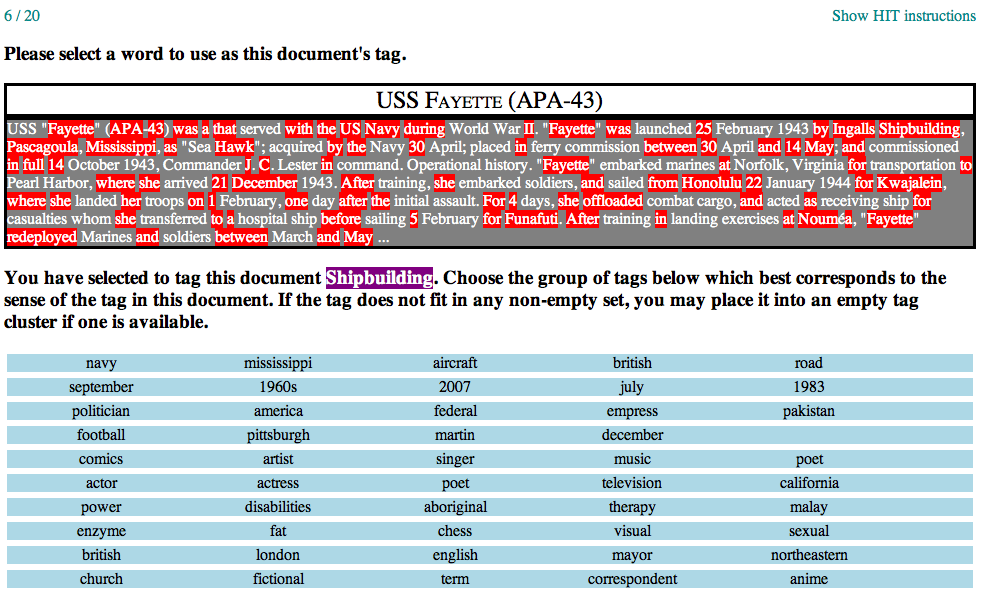
\includegraphics[width=0.90\textwidth]{figures/screenshots.png}
\caption{Screenshots of our task.  In the center, the document along
  with its title is shown.  Words which cannot be selected, e.g.,
  distractors and words previously selected, are shown in red.  Once a
  word is selected, the user is asked to find a topic in which to
  place the word.  The user selects a topic by clicking on an entry in
  a menu of topics, where each topic is expressed by the five words
  which occur most frequently in that topic.}
\label{fig:screenshot}
\end{figure*}

When the set of words minus the intruder makes sense together, then
the subject should easily identify the intruder.  For example, most
people readily identify \word{apple} as the intruding word in the set
\wordset{dog, cat, horse, apple, pig, cow} because the remaining
words, \wordset{dog, cat, horse, pig, cow} make sense together ---
they are all animals.  For the set \wordset{car, teacher, platypus,
  agile, blue, Zaire}, which lacks such coherence, identifying
the intruder is difficult.  People will typically choose an
intruder at random, implying a topic with poor coherence.

% sgerrish: I removed this paragraph, at least until we can measure this.
% The inter-subject agreement on the word intrusion task yields a
% measure of how semantically meaningful a set of words is: when all of
% the users agree on the intruder the set is semantically coherent; when
% none of them agree then the set is not.  

% jbg: I removed this footnote
% \footnote{The top words can be ranked either according to their
%   absolute probability mass in that topic, or according to their
%   probability mass in that topic relative to their unigram
%   probabilities.}

In order to construct a set to present to the subject, we first select
at random a topic from the model.  We then select the five most probable
words from that topic.  In addition to these words, an intruder word
is selected at random from a pool of words with low probability in the
current topic (to reduce the possibility that the intruder comes from
the same semantic group) but high probability in some other topic (to
ensure that the intruder is not rejected outright due solely to
rarity).  All six words are then shuffled and presented to the subject.

% In addition to being able to measure the semantic coherence of the
% topics using inter-subject agreement as described above, this task
% also enables the evaluation of whether the semantic divisions posited
% by a topic model correspond to those used by humans.  If the intruder
% as predicted by the topic model matched what the subjects thought was
% the intruder, then the topic found by the topic model resembles a set
% that our subjects believe is semantically coherent.

% While this
% approach also requires that models are able to select coherent topics,
% the first task provides an indication of whether the provided topics
% are reasonable.

For both the word intrusion and topic intrusion tasks, subjects were
instructed to focus on the meanings of words, not their syntactic
usage or orthography.  We also presented subjects with the option of
viewing the ``correct'' answer after they submitted their own
response, to make the tasks more engaging.  Here the ``correct''
answer was determined by the model which generated the data, presented
as if it were the response of another user.  At the same time,
subjects were encouraged to base their responses on their own
opinions, not to try to match other subjects' (the models')
selections.  In small experiments, we have found that this extra
information did not bias subjects' responses.


\section{Experimental results}
\label{sec:experiments}

We conducted our experiments using Amazon Mechanical
Turk~\footnote{http://www.mturk.com}, which allows workers (our pool
of prospective subjects) to perform small jobs for a fee through a Web
interface.  No specialized training or knowledge is typically expected
of the workers.  Amazon Mechanical Turk has been successfully used in
the past to develop gold-standard data for natural language
processing~\cite{snow-08} and to label images~\cite{imagenet-cvpr09}.

we prepare two randomly-chosen, 100-document subsets of English
Wikipedia~\footnote{http://en.wikipedia.org}.  For convenience, we
denote these two sets of documents as \emph{set1} and \emph{set2}.
For each document, we keep only the first 150 words for our
experiments.  Because of the encyclopedic nature of the corpus, the
first 150 words typically provides a broad overview of the themes in
the article.  We also removed from the corpus stop words and words
which occur infrequently\footnote{Infrequently occurring words were
  identified as those appearing fewer than eight times on a larger
  collection of 7726 articles.}, leading to a lexicon of 8263 words.
After this pruning \emph{set1} contained 11614 words and \emph{set2}
contained 11318 words.

Workers were asked to perform twenty of the taggings described in
\mysec{sec:tasks} for each task; workers were paid \$0.25 for each
such task.  The number of latent topics, $K$, is a free parameter.
Here we explore two values of this parameter, $K=10$ and $K=15$,
leading to a total of four experiments --- two for each set of
documents and two for each value of $K$.

\subsection{Tagging behavior}

There are several metrics commonly used to evaluate topic models in
the literature~\cite{wallach-09}.  Many of these metrics are
\emph{predictive} metrics; that is, they capture the model's ability
to predict a \emph{test set} of unseen documents after having learned
its parameters from a \emph{training set}.  In this work, we set aside
20\% of the documents in each corpus as a test set and train on the
remaining 80\% of documents.  We then compute predictive rank and
predictive log likelihood.

\begin{table*}
  \caption{The five words with the highest probability mass in each topic inferred by humans using the task described in \mysec{sec:tasks}.  Each subtable shows the results for a particular experimental setup.   Each row is a topic; the most probable words are ordered from left to right.}
\label{tab:topic-samples}
\centering
\footnotesize
\hspace*{-.4in}
\subfigure[\emph{set1}, $K = 10$]{
\begin{tabular}{lllll}
  railway & lighthouse & rail & huddersfield & station \\ 
  school & college & education & history & conference \\ 
  catholic & church & film & music & actor \\ 
  runners & team & championships & match & racing \\ 
  engine & company & power & dwight & engines \\ 
  university & london & british & college & county \\ 
  food & novel & book & series & superman \\ 
  november & february & april & august & december \\ 
  paint & photographs & american & austin & black \\ 
   war & history & army & american & battle \\ 
\end{tabular}
}%
\subfigure[\emph{set2}, $K = 10$]{
  \begin{tabular}{|lllll}
    president & emperor & politician & election & government \\ 
    american & players & swedish & team & zealand \\ 
    war & world & navy & road & torpedo \\ 
    system & pop & microsoft & music & singer \\ 
    september & 2007 & october & december & 1999 \\ 
    television & dog & name & george & film \\ 
    people & malay & town & tribes & cliff \\ 
    diet & chest & enzyme & hair & therapy \\ 
    british & city & london & english & county \\ 
    school & university & college & church & center \\ 
  \end{tabular}
}
\hspace*{-.5in}
\subfigure[\emph{set1}, $K = 15$]{
\begin{tabular}{lllll}
australia & knee & british & israel & set \\ 
  catholic & roman & island & village & columbia \\ 
  john & devon & michael & austin & charles \\ 
  school & university & class & community & district \\ 
  november & february & 2007 & 2009 & 2005 \\ 
  lighthouse & period & architects & construction & design \\ 
  railway & rail & huddersfield & ownership & services \\ 
  cyprus & archdiocese & diocese & king & miss \\ 
  carson & gordon & hugo & ward & whitney \\ 
  significant & application & campaign & comic & considered \\ 
  born & london & american & england & black \\ 
  war & defense & history & military & artillery \\ 
  actor & film & actress & band & designer \\ 
  york & michigan & florida & north & photographs \\ 
  church & catholic & county & 2001 & agricultural \\ 
\end{tabular}
}%
\subfigure[\emph{set2}, $K = 15$]{
\begin{tabular}{|lllll}
  music & pop & records & singer & artist \\ 
  film & paintings & movie & painting & art \\ 
  school & university & english & students & british \\ 
  drama & headquarters & chess & poet & stories \\ 
  family & church & sea & christmas & emperor \\ 
  dog & broadcast & television & bbc & breed \\ 
  champagne & regular & character & characteristic & common \\ 
  election & government & parliament & minister & politician \\ 
  enzyme & diet & protein & hair & oxygen \\ 
  war & navy & weapons & aircraft & military \\ 
  september & october & december & 2008 & 1967 \\ 
  district & town & marin & america & american \\ 
  car & power & system & device & devices \\ 
  hockey & players & football & therapy & champions \\ 
  california & zealand & georgia & india & kolkata \\ 
\end{tabular}
}
\vspace{0.2in}
\end{table*}

\begin{figure*}
\centering
\subfigure[$K = 10$]{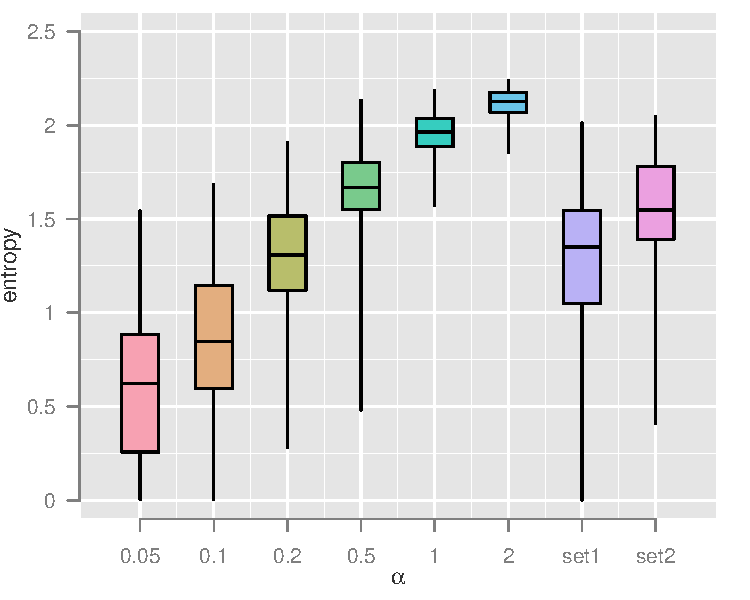
\includegraphics[width = .47\linewidth]{figures/entropy_K10}}%
\subfigure[$K = 15$]{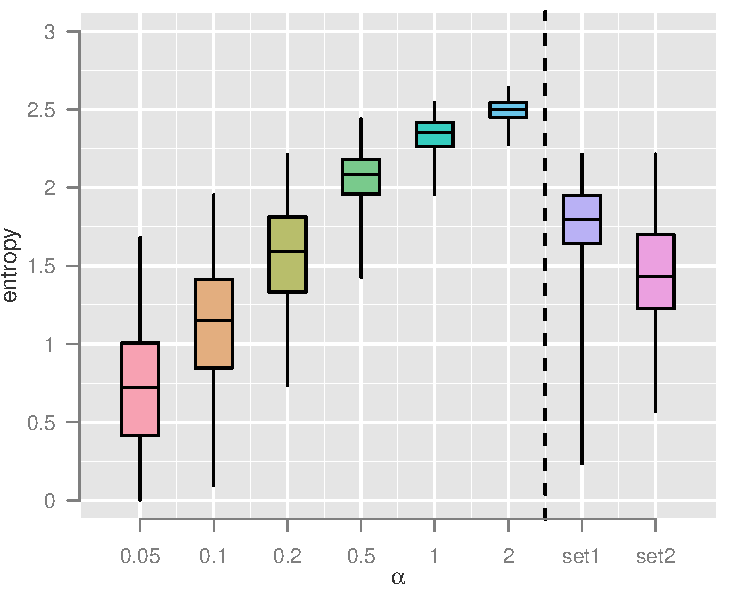
\includegraphics[width = .47\linewidth]{figures/entropy_K15}}

\caption{A comparison of the entropy of distributions drawn from a
  Dirichlet versus the entropy of the topic proportions inferred by
  workers.  Each column of the boxplot shows the distribution of
  entropies for 100 draws from a Dirichlet distribution with parameter
  $\alpha$.  The two rightmost columns show the distribution of the
  entropy of the topic proportions inferred by workers on \emph{set1}
  and \emph{set2}.  The $\alpha$ workers typically falls between 0.2
  and 0.5.}

\label{fig:entropy}
\end{figure*}

\subsection{Comparison with LDA}
\begin{figure*}
\centering
\subfigure[\emph{full}, $K = 10$]{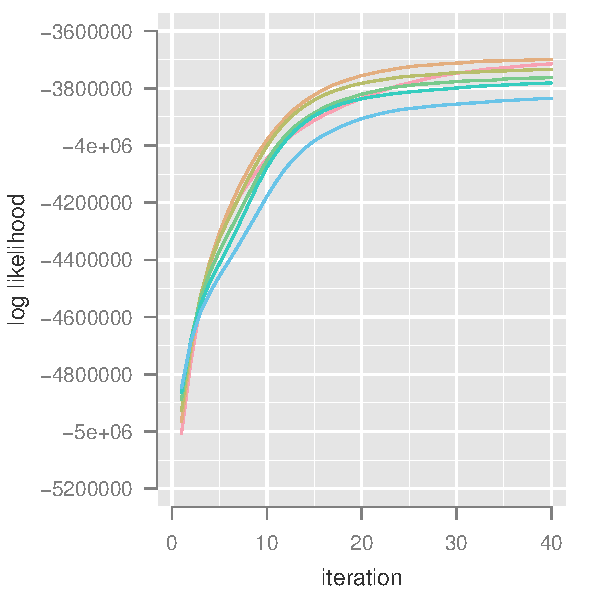
\includegraphics[width = .32\linewidth]{figures/lda_ll_full_10}}%
\subfigure[\emph{set1}, $K = 10$]{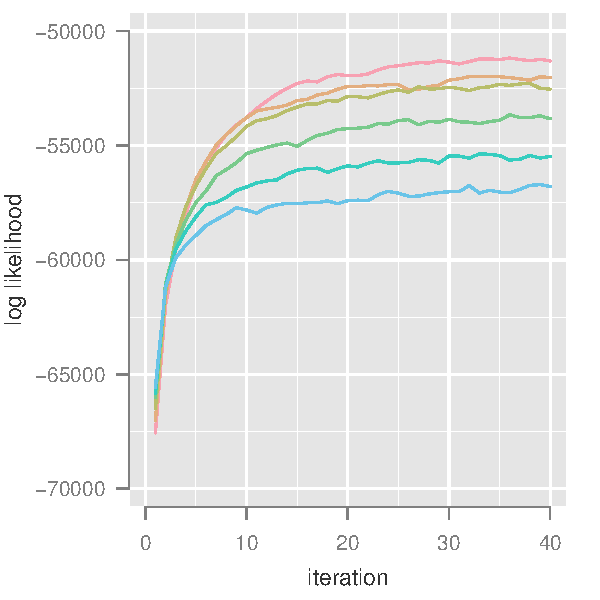
\includegraphics[width = .32\linewidth]{figures/lda_ll_set1_10}}%
\subfigure[\emph{set2}, $K = 10$]{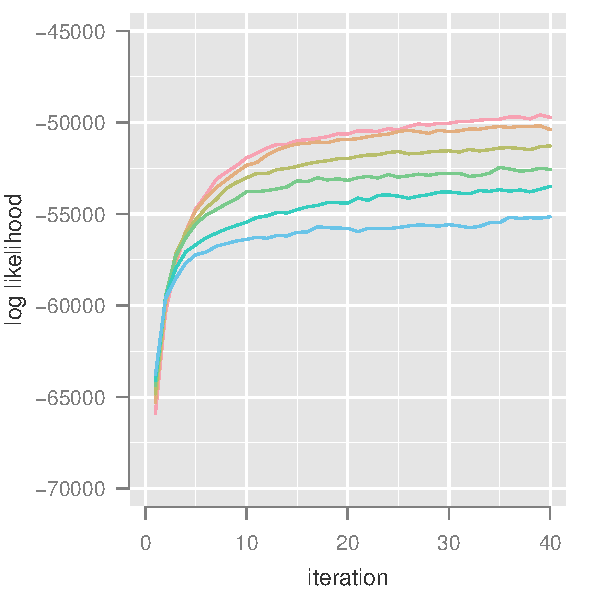
\includegraphics[width = .32\linewidth]{figures/lda_ll_set2_10}}

\subfigure[\emph{full}, $K = 15$]{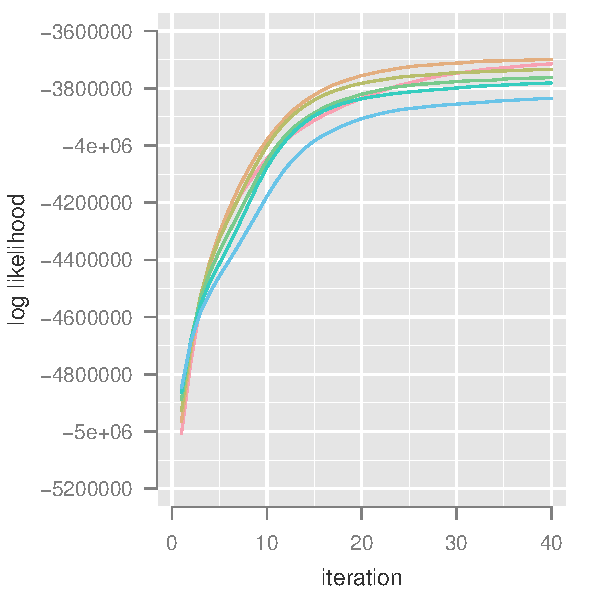
\includegraphics[width = .32\linewidth]{figures/lda_ll_full_10}}%
\subfigure[\emph{set1}, $K = 15$]{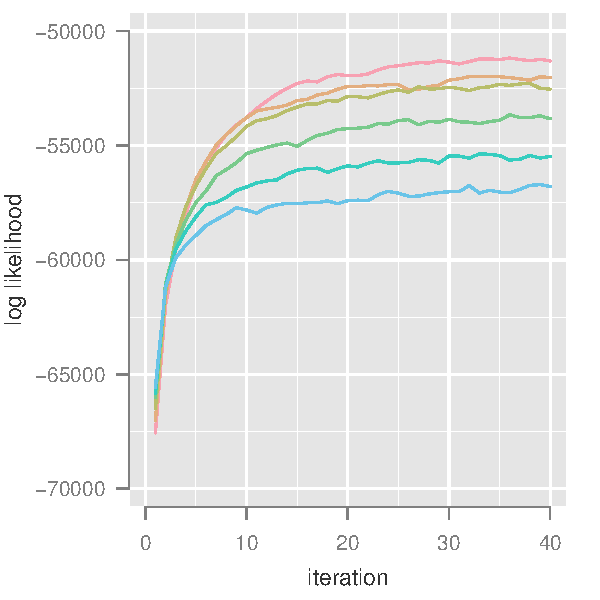
\includegraphics[width = .32\linewidth]{figures/lda_ll_set1_10}}%
\subfigure[\emph{set2}, $K = 15$]{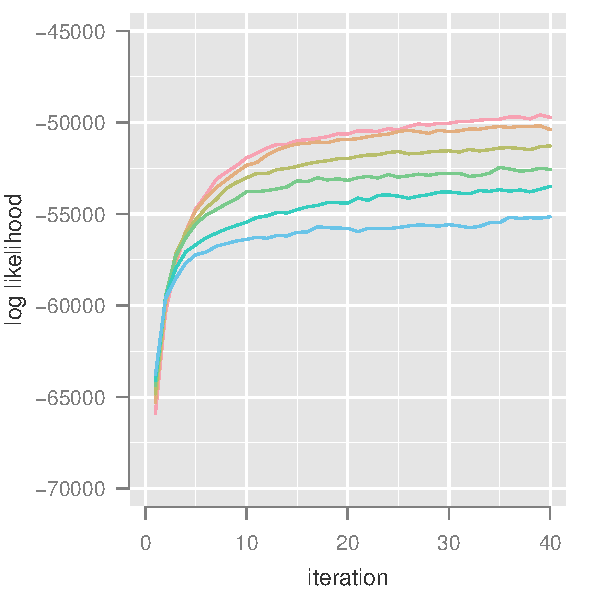
\includegraphics[width = .32\linewidth]{figures/lda_ll_set2_10}}

\caption{The log-likelihood achieved by LDA as a function of iteration.  \emph{full} refers to a larger set of 7726 Wikipedia articles.   There is one series for each value of $\alpha \in \{0.05, 0.1, 0.2, 0.5, 1.0, 2.0\}$ from top to bottom.}
\label{fig:ll}
\end{figure*}

\begin{table*}[ht]
\footnotesize
\centering
  \caption{The five words with the highest probability mass in each topic inferred by LDA.  Each subtable shows the results for a particular experimental setup.   Each row is a topic; the most probable words are ordered from left to right.}
\label{tab:lda-topic-samples}
\hspace*{-.1in}
\subfigure[\emph{set1}, $K=10$]{
\begin{tabular}{lllll}
born & 2004 & team & award & sydney \\ 
  regiment & army & artillery & served & scouting \\ 
  line & station & main & island & railway \\ 
  region & street & located & site & knee \\ 
  food & february & conference & day & 2009 \\ 
  pride & greek & knowledge & portland & study \\ 
  catholic & church & roman & black & time \\ 
  class & series & film & actor & engine \\ 
  travel & human & office & management & defense \\ 
  school & born & war & world & university \\ 
\end{tabular}
}%
\subfigure[\emph{set2}, $K=10$]{
\begin{tabular}{|lllll}
september & english & edit & nord & hockey \\ 
  black & hole & current & england & model \\ 
  training & program & war & election & navy \\ 
  school & university & district & city & college \\ 
  family & word & international & road & japan \\ 
  publication & time & day & india & bridge \\ 
  born & pop & world & released & march \\ 
  won & video & microsoft & project & hungary \\ 
  film & hair & bank & national & town \\ 
  people & name & french & therapy & artist \\ 
\end{tabular}
}
\hspace*{-.3in}
\subfigure[\emph{set1}, $K=15$]{
\begin{tabular}{lllll}
time & michael & written & experience & match \\ 
  line & station & railway & branch & knowledge \\ 
  film & land & pass & set & battle \\ 
  william & florida & carson & virginia & newfoundland \\ 
  war & regiment & british & army & south \\ 
  reaction & terminal & copper & running & complex \\ 
  born & school & world & college & black \\ 
  food & conference & flight & medium & rail \\ 
  township & scouting & census & square & county \\ 
  travel & defense & training & management & edges \\ 
  series & actor & engine & november & award \\ 
  pride & portland & band & northwest & god \\ 
  team & knee & 2004 & sydney & israel \\ 
  catholic & located & site & region & church \\ 
  class & february & time & public & king \\ 
\end{tabular}
}%
\subfigure[\emph{set2}, $K=15$]{
\begin{tabular}{|lllll}
family & protein & enzyme & acting & oxygen \\ 
  england & producer & popular & canadian & sea \\ 
  system & death & artist & running & car \\ 
  character & series & dark & main & village \\ 
  english & word & publication & stream & day \\ 
  training & program & hair & students & electrical \\ 
  district & town & city & local & kolkata \\ 
  september & edit & music & records & recorded \\ 
  black & pop & bank & usually & hole \\ 
  people & choir & road & diet & related \\ 
  war & built & navy & british & service \\ 
  center & million & cut & champagne & players \\ 
  born & television & current & drama & won \\ 
  school & university & college & election & born \\ 
  film & nord & played & league & hockey \\ 
\end{tabular}
}
\end{table*}

As described in \mysec{sec:wordintrusion}, the word intrusion task
measures how well the inferred topics match human concepts (using
\emph{model precision}, i.e., how well the intruders detected by the
subjects correspond to those injected into ones found by the topic
model).

\myfig{fig:precision} shows boxplots of the precision for the three
models on the two corpora.  In most cases LDA performs best. Although
CTM gives better predictive results on held-out likelihood, it does
not perform as well on human evaluations. This may be because CTM
finds correlations between topics and correlations within topics are
confounding factors; the intruder for one topic might be selected from
another highly correlated topic.  The performance of pLSI degrades
with larger numbers of topics, suggesting that
overfitting~\cite{blei-03} might affect interpretability as well as
predictive power.

\myfig{fig:topic_precision} (left) shows examples of topics with high
and low model precisions from the NY Times data fit with LDA using 50
topics. In the example with high precision, the topic words all
coherently express a painting theme.  For the low precision example,
``taxis'' did not fit in with the other political words in the topic,
as $87.5\%$ of subjects chose ``taxis'' as the intruder.




\section{Discussion}
  We presented the first method for constructing topic models using
  human judgments.  Our approach relies on a novel task,
  \emph{tag-and-cluster}, which asks users to simultanesouly annotate
  a document with one of its words and to cluster those annotations.
  We demonstrate using experiments on Amazon Mechanical Turk that our
  method constructs topic models quickly and robustly.  We also show
  that while our topic models bear many similarities to traditionally
  constructed topic models, our human-learned topic models have unique
  features such as fixed sparsity and a tendency to construct topics
  around concepts which models such as LDA typically fail to find.

  We also underscore that the collapsed Gibbs sampling framework is
  expressive enough to use as the basis for human-guided topic model
  inference.  This may motivate, as future work, the construction of
  different modeling assumptions which lead to sampling equations
  which more closely match the empirically observed sampling performed
  by humans.  In effect, our method constructs a series of samples
  from the posterior, a gold standard which future topic models can
  aim to emulate.
\bibliographystyle{naaclhlt2010}

\small

\bibliography{journal-abbrv,nlp}

\end{document}
